\section{Behavioural-Vs-Vendor Agreement and Applicability Boundary}

The behavioural-vs-vendor agreement analysis is the main boundary-finding result in this report. Agreement is strongest for moderate and larger $C_f$ values, where the compensation choice lowers bandwidth and suppresses peaking enough for the single-pole behavioural model to track the broad vendor-export trend. Agreement degrades in small-$C_f$ cases, where the closed-loop bandwidth approaches op-amp bandwidth limits and omitted higher-order vendor macromodel dynamics become more visible (Figure~\ref{fig:model-agreement-error-summary}; Table~\ref{tab:agreement-summary}).

The label count remains useful but secondary: across the 11 selected OP27, OPA818, and ADA4817 cases, 9 project-defined labels agree between the MATLAB behavioural model and the vendor macromodel summaries. For OPA818, label agreement is obtained in all four rows, but bandwidth error is largest at $C_f=0.5$ pF and decreases for larger $C_f$. For ADA4817, the larger-$C_f$ cases agree in the project-defined label comparison, while the $C_f=0.5$ pF row remains a disagreement case because the vendor macromodel reports peaking that the simplified behavioural model does not reproduce. For OP27, the smallest-$C_f$ row demonstrates the low-GBW negative-control limitation: the vendor summary labels the case Risky, while the MATLAB behavioural model labels it Safe under the project-defined peaking criterion. The corresponding small-$C_f$ overlays are included in the appendix (Figures~\ref{fig:appendix-opa818-small-cf-overlay}--\ref{fig:appendix-op27-small-cf-overlay}).

The input-capacitance ablation does not support a blanket claim that adding input capacitance improves agreement. Across all 11 rows, mean absolute bandwidth error changes from 18.83\% without $C_{in}$ to 19.33\% with documented $C_{in}$, and label agreement remains 9/11. For the high-speed OPA818 and ADA4817 rows together, mean absolute bandwidth error changes from 17.29\% to 17.96\%. ADA4817 improves modestly, while OPA818 worsens under the current assumptions. This mixed result is consistent with the tested vendor rows using $C_{pd}=10$ pF, which dominates the documented $C_{in}$ values.

The practical interpretation is therefore conditional. Labels in moderate-to-large-$C_f$ cases can be used for fast triage and prioritisation, provided they remain tied to the stated repository assumptions. Labels in the small-$C_f$ bandwidth-limited corner should be treated as provisional and reviewed with detailed vendor macromodel or SPICE evidence before design decisions are made.

\AgreementSummaryTable

\begin{figure}[H]
  \centering
  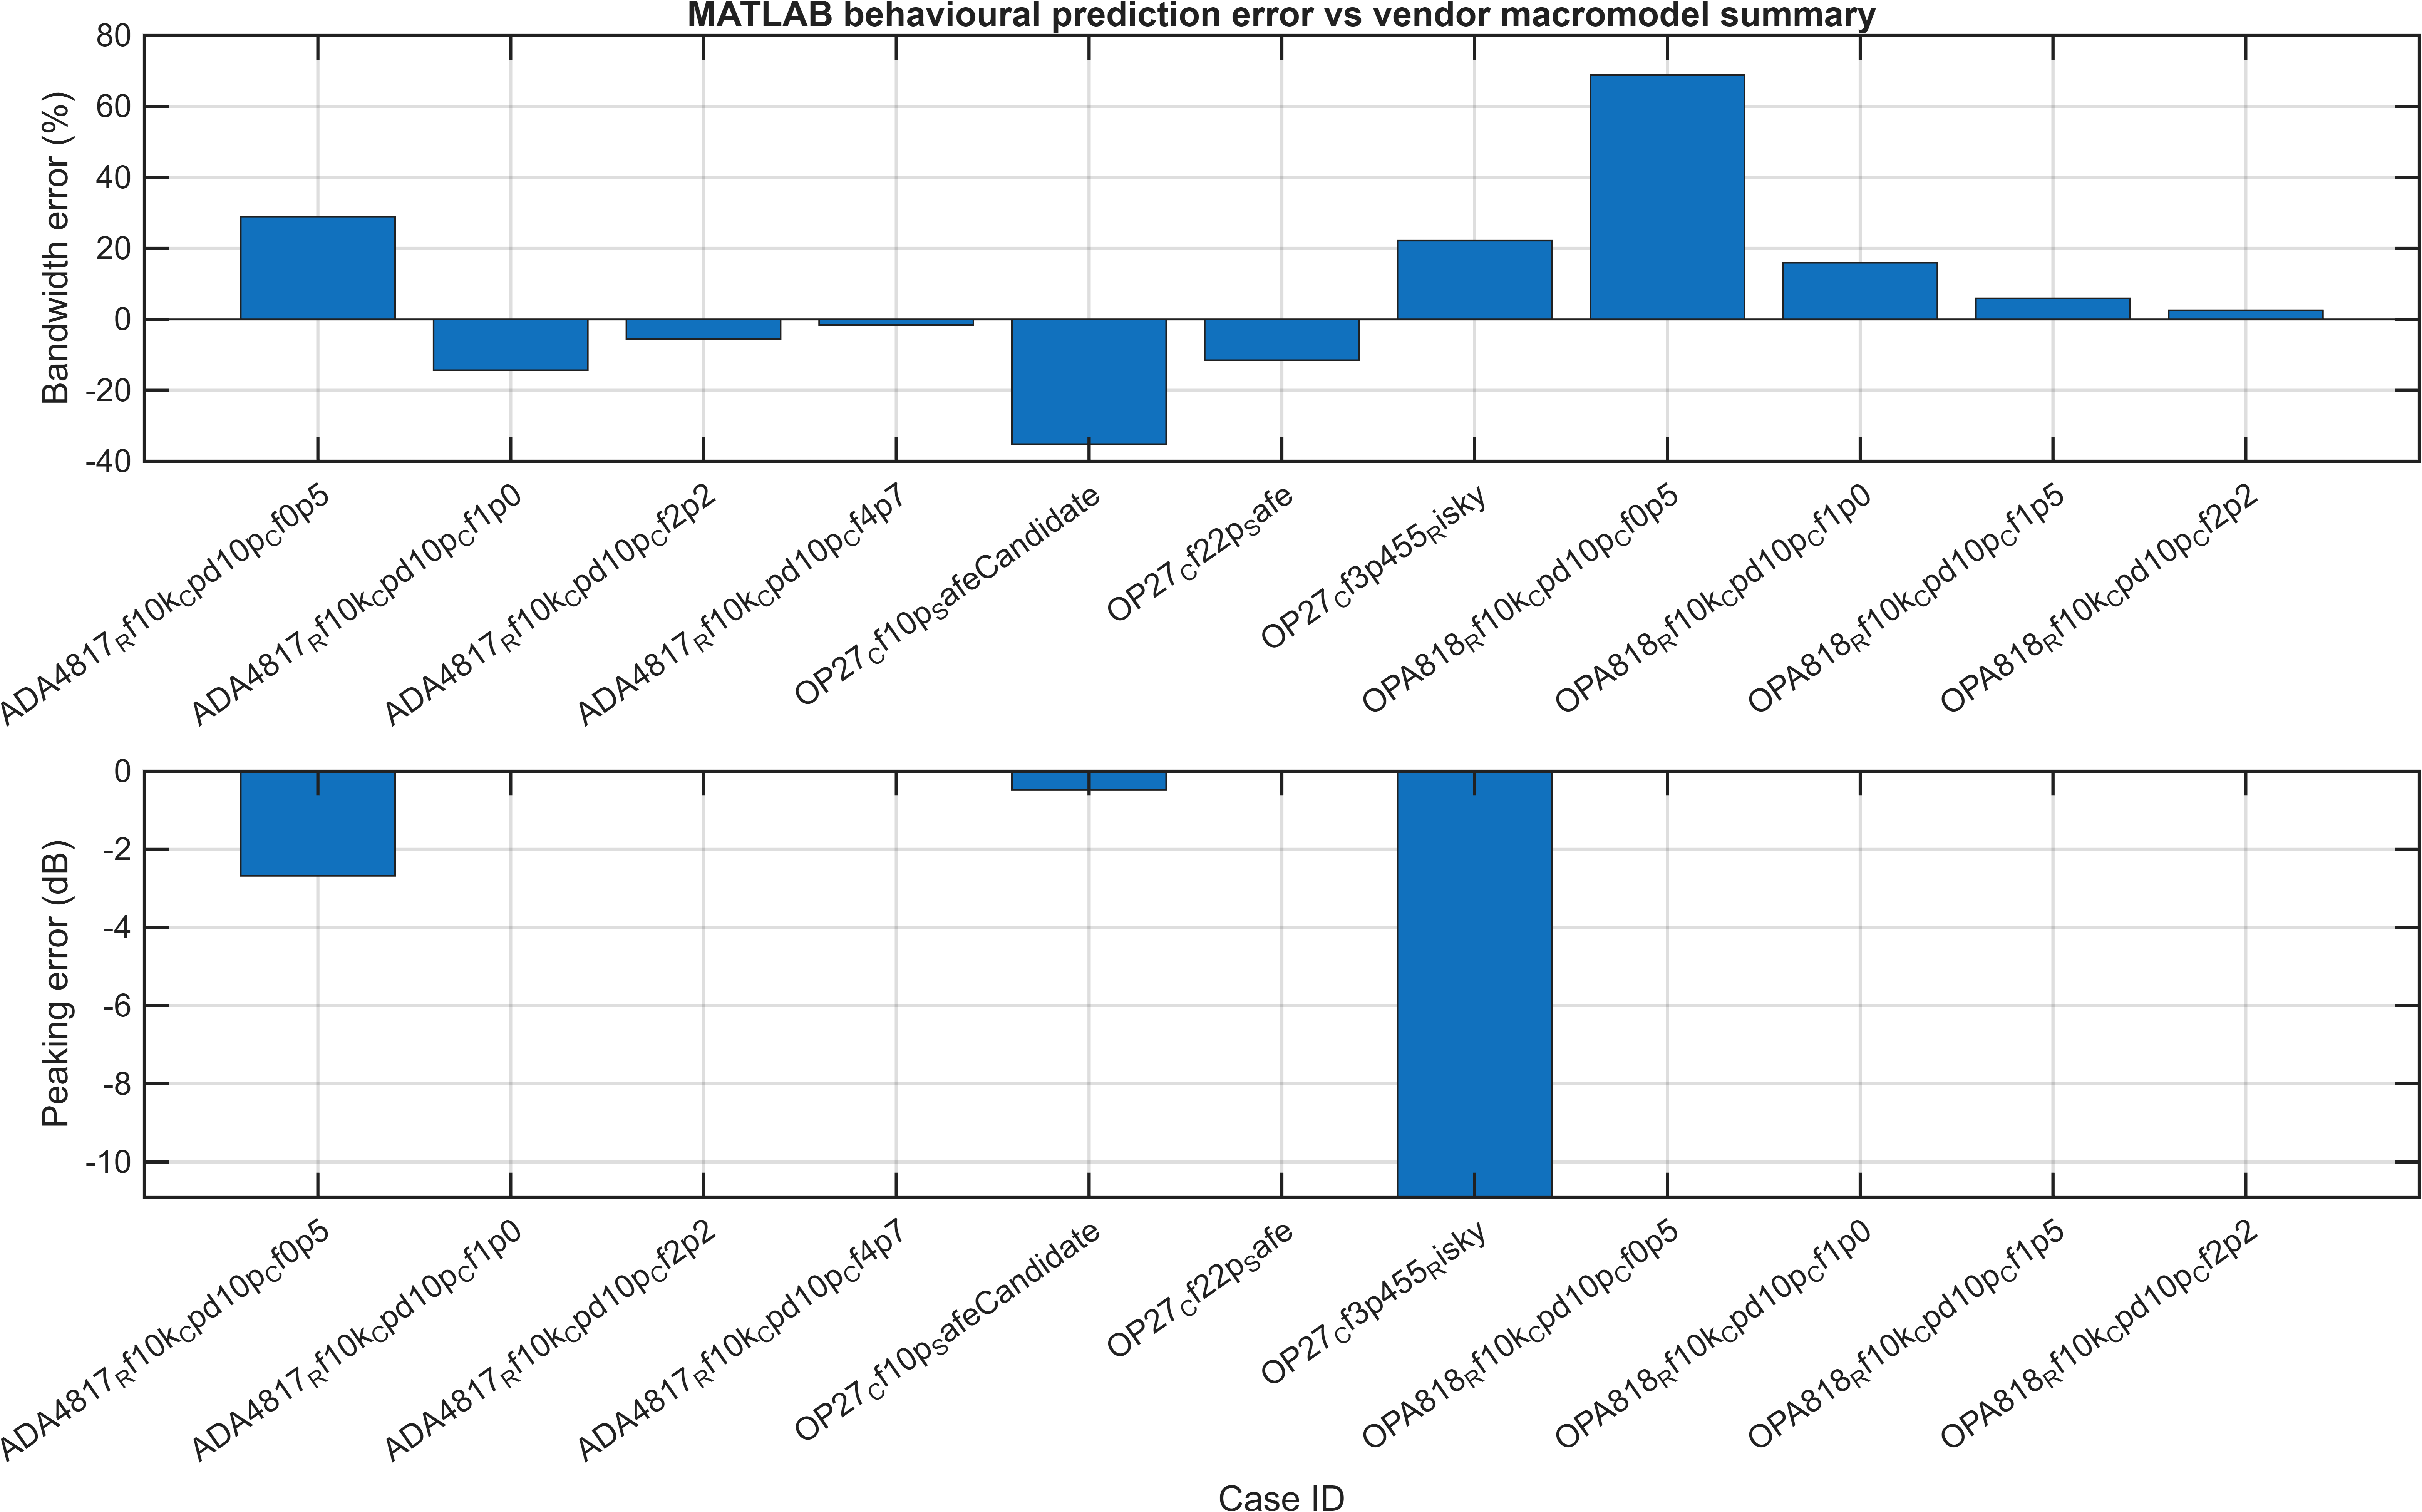
\includegraphics[width=0.84\linewidth]{figures/behavioural_vs_vendor_agreement_error_summary.png}
  \caption{Behavioural-vs-vendor-macromodel agreement error summary for OP27, OPA818, and ADA4817 feedback-capacitance cases. Bandwidth error is computed as $100(\mathrm{MATLAB}-\mathrm{vendor})/\mathrm{vendor}$, and peaking error is MATLAB peaking minus vendor peaking.}
  \label{fig:model-agreement-error-summary}
\end{figure}
\FloatBarrier
